\documentclass[]{article}
\usepackage{lmodern}
\usepackage{amssymb,amsmath}
\usepackage{ifxetex,ifluatex}
\usepackage{fixltx2e} % provides \textsubscript
\ifnum 0\ifxetex 1\fi\ifluatex 1\fi=0 % if pdftex
  \usepackage[T1]{fontenc}
  \usepackage[utf8]{inputenc}
\else % if luatex or xelatex
  \ifxetex
    \usepackage{mathspec}
  \else
    \usepackage{fontspec}
  \fi
  \defaultfontfeatures{Ligatures=TeX,Scale=MatchLowercase}
\fi
% use upquote if available, for straight quotes in verbatim environments
\IfFileExists{upquote.sty}{\usepackage{upquote}}{}
% use microtype if available
\IfFileExists{microtype.sty}{%
\usepackage{microtype}
\UseMicrotypeSet[protrusion]{basicmath} % disable protrusion for tt fonts
}{}
\usepackage[margin=1in]{geometry}
\usepackage{hyperref}
\hypersetup{unicode=true,
            pdftitle={main.java.spamizer},
            pdfauthor={Marc Sànchez, Francesc Xavier Bullich, Gil Gassó},
            pdfborder={0 0 0},
            breaklinks=true}
\urlstyle{same}  % don't use monospace font for urls
\usepackage{color}
\usepackage{fancyvrb}
\newcommand{\VerbBar}{|}
\newcommand{\VERB}{\Verb[commandchars=\\\{\}]}
\DefineVerbatimEnvironment{Highlighting}{Verbatim}{commandchars=\\\{\}}
% Add ',fontsize=\small' for more characters per line
\usepackage{framed}
\definecolor{shadecolor}{RGB}{248,248,248}
\newenvironment{Shaded}{\begin{snugshade}}{\end{snugshade}}
\newcommand{\AlertTok}[1]{\textcolor[rgb]{0.94,0.16,0.16}{#1}}
\newcommand{\AnnotationTok}[1]{\textcolor[rgb]{0.56,0.35,0.01}{\textbf{\textit{#1}}}}
\newcommand{\AttributeTok}[1]{\textcolor[rgb]{0.77,0.63,0.00}{#1}}
\newcommand{\BaseNTok}[1]{\textcolor[rgb]{0.00,0.00,0.81}{#1}}
\newcommand{\BuiltInTok}[1]{#1}
\newcommand{\CharTok}[1]{\textcolor[rgb]{0.31,0.60,0.02}{#1}}
\newcommand{\CommentTok}[1]{\textcolor[rgb]{0.56,0.35,0.01}{\textit{#1}}}
\newcommand{\CommentVarTok}[1]{\textcolor[rgb]{0.56,0.35,0.01}{\textbf{\textit{#1}}}}
\newcommand{\ConstantTok}[1]{\textcolor[rgb]{0.00,0.00,0.00}{#1}}
\newcommand{\ControlFlowTok}[1]{\textcolor[rgb]{0.13,0.29,0.53}{\textbf{#1}}}
\newcommand{\DataTypeTok}[1]{\textcolor[rgb]{0.13,0.29,0.53}{#1}}
\newcommand{\DecValTok}[1]{\textcolor[rgb]{0.00,0.00,0.81}{#1}}
\newcommand{\DocumentationTok}[1]{\textcolor[rgb]{0.56,0.35,0.01}{\textbf{\textit{#1}}}}
\newcommand{\ErrorTok}[1]{\textcolor[rgb]{0.64,0.00,0.00}{\textbf{#1}}}
\newcommand{\ExtensionTok}[1]{#1}
\newcommand{\FloatTok}[1]{\textcolor[rgb]{0.00,0.00,0.81}{#1}}
\newcommand{\FunctionTok}[1]{\textcolor[rgb]{0.00,0.00,0.00}{#1}}
\newcommand{\ImportTok}[1]{#1}
\newcommand{\InformationTok}[1]{\textcolor[rgb]{0.56,0.35,0.01}{\textbf{\textit{#1}}}}
\newcommand{\KeywordTok}[1]{\textcolor[rgb]{0.13,0.29,0.53}{\textbf{#1}}}
\newcommand{\NormalTok}[1]{#1}
\newcommand{\OperatorTok}[1]{\textcolor[rgb]{0.81,0.36,0.00}{\textbf{#1}}}
\newcommand{\OtherTok}[1]{\textcolor[rgb]{0.56,0.35,0.01}{#1}}
\newcommand{\PreprocessorTok}[1]{\textcolor[rgb]{0.56,0.35,0.01}{\textit{#1}}}
\newcommand{\RegionMarkerTok}[1]{#1}
\newcommand{\SpecialCharTok}[1]{\textcolor[rgb]{0.00,0.00,0.00}{#1}}
\newcommand{\SpecialStringTok}[1]{\textcolor[rgb]{0.31,0.60,0.02}{#1}}
\newcommand{\StringTok}[1]{\textcolor[rgb]{0.31,0.60,0.02}{#1}}
\newcommand{\VariableTok}[1]{\textcolor[rgb]{0.00,0.00,0.00}{#1}}
\newcommand{\VerbatimStringTok}[1]{\textcolor[rgb]{0.31,0.60,0.02}{#1}}
\newcommand{\WarningTok}[1]{\textcolor[rgb]{0.56,0.35,0.01}{\textbf{\textit{#1}}}}
\usepackage{graphicx,grffile}
\makeatletter
\def\maxwidth{\ifdim\Gin@nat@width>\linewidth\linewidth\else\Gin@nat@width\fi}
\def\maxheight{\ifdim\Gin@nat@height>\textheight\textheight\else\Gin@nat@height\fi}
\makeatother
% Scale images if necessary, so that they will not overflow the page
% margins by default, and it is still possible to overwrite the defaults
% using explicit options in \includegraphics[width, height, ...]{}
\setkeys{Gin}{width=\maxwidth,height=\maxheight,keepaspectratio}
\IfFileExists{parskip.sty}{%
\usepackage{parskip}
}{% else
\setlength{\parindent}{0pt}
\setlength{\parskip}{6pt plus 2pt minus 1pt}
}
\setlength{\emergencystretch}{3em}  % prevent overfull lines
\providecommand{\tightlist}{%
  \setlength{\itemsep}{0pt}\setlength{\parskip}{0pt}}
\setcounter{secnumdepth}{0}
% Redefines (sub)paragraphs to behave more like sections
\ifx\paragraph\undefined\else
\let\oldparagraph\paragraph
\renewcommand{\paragraph}[1]{\oldparagraph{#1}\mbox{}}
\fi
\ifx\subparagraph\undefined\else
\let\oldsubparagraph\subparagraph
\renewcommand{\subparagraph}[1]{\oldsubparagraph{#1}\mbox{}}
\fi

%%% Use protect on footnotes to avoid problems with footnotes in titles
\let\rmarkdownfootnote\footnote%
\def\footnote{\protect\rmarkdownfootnote}

%%% Change title format to be more compact
\usepackage{titling}

% Create subtitle command for use in maketitle
\providecommand{\subtitle}[1]{
  \posttitle{
    \begin{center}\large#1\end{center}
    }
}

\setlength{\droptitle}{-2em}

  \title{main.java.spamizer}
    \pretitle{\vspace{\droptitle}\centering\huge}
  \posttitle{\par}
    \author{Marc Sànchez, Francesc Xavier Bullich, Gil Gassó}
    \preauthor{\centering\large\emph}
  \postauthor{\par}
      \predate{\centering\large\emph}
  \postdate{\par}
    \date{5/8/2019}


\begin{document}
\maketitle

\newpage

// TODO : Posar el projecte al github.

\begin{Shaded}
\begin{Highlighting}[]
\CommentTok{# x és el nom del fitxer que volem carregar}
\NormalTok{loadFormattedData <-}\StringTok{ }\ControlFlowTok{function}\NormalTok{(x)\{}
  
\NormalTok{  tmp =}\StringTok{ }\KeywordTok{read.csv}\NormalTok{(x)}
  \KeywordTok{names}\NormalTok{(tmp) <-}\StringTok{ }\KeywordTok{c}\NormalTok{(}\StringTok{"id"}\NormalTok{, }\StringTok{"phi"}\NormalTok{, }\StringTok{"k"}\NormalTok{, }\StringTok{"tp"}\NormalTok{, }\StringTok{"tn"}\NormalTok{, }\StringTok{"fp"}\NormalTok{, }\StringTok{"fn"}\NormalTok{, }\StringTok{"nham"}\NormalTok{, }\StringTok{"nspam"}\NormalTok{)}
  
  \CommentTok{#Calculem els tcr dels valors }
  \CommentTok{# BASE :  (NSPAM) / (50 * NHAM + NSPAM) }
\NormalTok{  base <-}\StringTok{ }\NormalTok{tmp}\OperatorTok{$}\NormalTok{nspam }\OperatorTok{/}\StringTok{ }\NormalTok{(}\DecValTok{50} \OperatorTok{*}\StringTok{ }\NormalTok{tmp}\OperatorTok{$}\NormalTok{nham }\OperatorTok{+}\StringTok{ }\NormalTok{tmp}\OperatorTok{$}\NormalTok{nspam)}
  \CommentTok{# WERR: (50 * FP + FN)/(50 * NHAM + NSPAM) + 0.000001 -> per que no sigui 0}
\NormalTok{  werr <-}\StringTok{ }\NormalTok{(}\DecValTok{50} \OperatorTok{*}\StringTok{ }\NormalTok{tmp}\OperatorTok{$}\NormalTok{fp }\OperatorTok{+}\StringTok{ }\NormalTok{tmp}\OperatorTok{$}\NormalTok{fn) }\OperatorTok{/}\StringTok{ }\NormalTok{(}\DecValTok{50} \OperatorTok{*}\StringTok{ }\NormalTok{tmp}\OperatorTok{$}\NormalTok{nham }\OperatorTok{+}\StringTok{ }\NormalTok{tmp}\OperatorTok{$}\NormalTok{nspam) }\OperatorTok{+}\StringTok{ }\FloatTok{0.000001}
  \CommentTok{# TCR : BASE / WERR}
\NormalTok{  tcr <-}\StringTok{ }\NormalTok{base}\OperatorTok{/}\NormalTok{werr}
  
  \CommentTok{# Calculem l'accuracy}
\NormalTok{  accuracy <-}\StringTok{ }\NormalTok{(tmp}\OperatorTok{$}\NormalTok{nspam }\OperatorTok{+}\StringTok{ }\NormalTok{tmp}\OperatorTok{$}\NormalTok{nham }\OperatorTok{-}\StringTok{ }\NormalTok{tmp}\OperatorTok{$}\NormalTok{fp }\OperatorTok{-}\StringTok{ }\NormalTok{tmp}\OperatorTok{$}\NormalTok{fn)}\OperatorTok{/}\NormalTok{(tmp}\OperatorTok{$}\NormalTok{nspam }\OperatorTok{+}\StringTok{ }\NormalTok{tmp}\OperatorTok{$}\NormalTok{nham) }\OperatorTok{*}\StringTok{ }\DecValTok{100}
  
  \CommentTok{# Generar una matriu que permeti representar els resultats en funció de k i phi}
\NormalTok{  values <-}\StringTok{ }\KeywordTok{data.frame}\NormalTok{(accuracy, tcr)}
  \KeywordTok{names}\NormalTok{(values) <-}\StringTok{ }\KeywordTok{c}\NormalTok{(}\StringTok{"accuracy"}\NormalTok{, }\StringTok{"tcr"}\NormalTok{)}
  \KeywordTok{head}\NormalTok{(values)}
  
\NormalTok{  tmp <-}\StringTok{ }\KeywordTok{cbind}\NormalTok{(tmp, values)}
  
  \CommentTok{# Ordenem els valors}
\NormalTok{  tmp <-}\StringTok{ }\NormalTok{tmp[}\KeywordTok{order}\NormalTok{(}\OperatorTok{-}\NormalTok{tmp}\OperatorTok{$}\NormalTok{tcr), ]}

   \KeywordTok{return}\NormalTok{(tmp)}
\NormalTok{\}}
\end{Highlighting}
\end{Shaded}

\hypertarget{naive-bayes}{%
\section{Naive Bayes}\label{naive-bayes}}

En aquest apartat s'especifica com s'adapta el mètode de naive bayes al
filtratge de correu.

\hypertarget{naive-bayes.}{%
\subsection{Naive Bayes.}\label{naive-bayes.}}

// TODO : S'ha de parlar de tot el que es fa a dins del mètode que tenim
implementat al codi.

\hypertarget{assumpcions.}{%
\subsection{Assumpcions.}\label{assumpcions.}}

// TODO : Comentar tot el que es dona per sentat al utilitzar aquest
mètode, com per exemple que la màquina està ben entrenada \ldots{}

\hypertarget{punts-forts-i-febles-del-metode-de-naive-bayes.}{%
\subsection{Punts forts i febles del mètode de Naive
Bayes.}\label{punts-forts-i-febles-del-metode-de-naive-bayes.}}

// TODO :

\hypertarget{applicacio.}{%
\section{Applicació.}\label{applicacio.}}

En aquest apartat s'es

\hypertarget{tecnologies-escollides.}{%
\subsection{Tecnologies escollides.}\label{tecnologies-escollides.}}

Comentar també la comparació de l'ús de base de dades en memòria.

\hypertarget{manual-de-laplicacio.}{%
\subsection{Manual de l'aplicació.}\label{manual-de-laplicacio.}}

\begin{Shaded}
\begin{Highlighting}[]
\CommentTok{# usage: main.java.spamizer}
\CommentTok{#  -c <arg>   Usage : -c <spamDir> <hamDir> [-n <int>]}
\CommentTok{#             Receives 2 parameters, A directory with spam mails and a}
\CommentTok{#             directory with ham mails. A calculation for values phi and k}
\CommentTok{#             will be done using a selection for the mails set. By default}
\CommentTok{#             the selection will be random based on k-fold cross-validation}
\CommentTok{#             and the heuristic method used to calculate phi and k values}
\CommentTok{#             will be random}
\CommentTok{#  -d         Flag that indicates that data must be loaded from local}
\CommentTok{#             database, this database is allocated inside project dir named}
\CommentTok{#             db made by csv files}
\CommentTok{#  -h         Set training mails as ham, adding this argument -s must not be}
\CommentTok{#             present}
\CommentTok{#  -n <arg>   The number of iterations for -c mode execution.}
\CommentTok{#  -p         Set the persistance of the memory database to a local database}
\CommentTok{#  -s         Set training mails as spam, adding this argument -h must not}
\CommentTok{#             be present}
\CommentTok{#  -t <arg>   Directories where training mails in txt are stored, this or}
\CommentTok{#             database argument must be present you can set a maximum of 2}
\CommentTok{#             directories in this several order : -t <spamDir> <hamDir>. If}
\CommentTok{#             only one dir is set the parameter -h or -s must be included}
\CommentTok{#  -v <arg>   Directory where validation mails in txt are stored. This}
\CommentTok{#             procedure will validate mail inside validationDir with}
\CommentTok{#             database loaded by default or stored inside memory. [-h | -s]}
\CommentTok{#             -v <validationDir> .}
\end{Highlighting}
\end{Shaded}

\hypertarget{utilitzacio.}{%
\subsection{Utilització.}\label{utilitzacio.}}

\hypertarget{implementacio.}{%
\section{Implementació.}\label{implementacio.}}

\hypertarget{lectura-de-fitxers.}{%
\subsection{Lectura de fitxers.}\label{lectura-de-fitxers.}}

\hypertarget{metode-de-seleccio.}{%
\subsection{Mètode de selecció.}\label{metode-de-seleccio.}}

\hypertarget{adaptacio-del-metode-k-fold-cross-validation.}{%
\subsubsection{Adaptació del mètode K-fold
cross-validation.}\label{adaptacio-del-metode-k-fold-cross-validation.}}

En comptes de realitzar la divisió \ldots{}

\hypertarget{filtre-i-abstraccio-del-filtratge.}{%
\subsection{Filtre i abstracció del
filtratge.}\label{filtre-i-abstraccio-del-filtratge.}}

\hypertarget{stanford-core-nlp.}{%
\subsubsection{Stanford Core NLP.}\label{stanford-core-nlp.}}

\hypertarget{custom-filter.}{%
\subsubsection{Custom Filter.}\label{custom-filter.}}

\hypertarget{entrenament.}{%
\subsection{Entrenament.}\label{entrenament.}}

\hypertarget{validacio.}{%
\subsection{Validació.}\label{validacio.}}

// TODO : Explicar la nostre adaptació del mètode hill climbing
utilitzat.

\hypertarget{compute-application-adaptacio-del-metode-hill-climbing.}{%
\subsection{Compute (main.java.Application, adaptació del mètode Hill
Climbing).}\label{compute-application-adaptacio-del-metode-hill-climbing.}}

\hypertarget{fase-experimental.}{%
\section{Fase Experimental.}\label{fase-experimental.}}

// TODO : \ldots{} Pensar l'estructura encara.

\hypertarget{evaluacio-dels-fp-i-dels-fn-en-funcio-de-k-i-phi}{%
\subsection{Evaluació dels FP i dels FN en funció de K i
PHI}\label{evaluacio-dels-fp-i-dels-fn-en-funcio-de-k-i-phi}}

// TODO :

\hypertarget{calcul-del-tcr-total-cost-ratio}{%
\subsection{Càlcul del TCR (Total Cost
Ratio)}\label{calcul-del-tcr-total-cost-ratio}}

Amb el Total cost ratio podem extreure un valor que pondera amb més
força el valor de les aparicions dels falços positius. El que es busca
amb el Tcr és el valor màxim possibles. Per fer-ho hem realitzat vàries
execucions i hem preparat una série de conclusions per intentar esbrinar
les funcions phi i k que millor s'acosten al nostre problema mitjançant
el càlcul del tcr.

\hypertarget{veiem-com-es-pot-generar-la-columna-tcr}{%
\subsubsection{Veiem com es pot generar la columna
TCR}\label{veiem-com-es-pot-generar-la-columna-tcr}}

\begin{Shaded}
\begin{Highlighting}[]
\NormalTok{results =}\StringTok{ }\KeywordTok{read.csv}\NormalTok{(}\StringTok{"./20000m-500n-SF.csv"}\NormalTok{)}
\CommentTok{#Calculem els tcr dels valors }
\CommentTok{# BASE :  (NSPAM) / (50 * NHAM + NSPAM) }
\NormalTok{base <-}\StringTok{ }\NormalTok{results}\OperatorTok{$}\NormalTok{NSPAM }\OperatorTok{/}\StringTok{ }\NormalTok{(}\DecValTok{50} \OperatorTok{*}\StringTok{ }\NormalTok{results}\OperatorTok{$}\NormalTok{NHAM }\OperatorTok{+}\StringTok{ }\NormalTok{results}\OperatorTok{$}\NormalTok{NSPAM)}
\CommentTok{# WERR: (50 * FP + FN)/(50 * NHAM + NSPAM) + 0.000001 -> per que no sigui 0}
\NormalTok{werr <-}\StringTok{ }\NormalTok{(}\DecValTok{50} \OperatorTok{*}\StringTok{ }\NormalTok{results}\OperatorTok{$}\NormalTok{FP }\OperatorTok{+}\StringTok{ }\NormalTok{results}\OperatorTok{$}\NormalTok{FN) }\OperatorTok{/}\StringTok{ }\NormalTok{(}\DecValTok{50} \OperatorTok{*}\StringTok{ }\NormalTok{results}\OperatorTok{$}\NormalTok{NHAM }\OperatorTok{+}\StringTok{ }\NormalTok{results}\OperatorTok{$}\NormalTok{NSPAM) }\OperatorTok{+}\StringTok{ }\FloatTok{0.000001}
\CommentTok{# TCR : BASE / WERR}
\NormalTok{tcr <-}\StringTok{ }\NormalTok{base}\OperatorTok{/}\NormalTok{werr}

\CommentTok{# Generar una matriu que permeti representar els resultats en funció de k i phi}
\NormalTok{values <-}\StringTok{ }\KeywordTok{data.frame}\NormalTok{(results}\OperatorTok{$}\NormalTok{PHI, results}\OperatorTok{$}\NormalTok{K, tcr)}
\KeywordTok{names}\NormalTok{(values) <-}\StringTok{ }\KeywordTok{c}\NormalTok{(}\StringTok{"phi"}\NormalTok{, }\StringTok{"k"}\NormalTok{, }\StringTok{"tcr"}\NormalTok{)}
\KeywordTok{head}\NormalTok{(values)}
\end{Highlighting}
\end{Shaded}

\begin{verbatim}
##        phi         k       tcr
## 1 2.103004 0.8211889 29.954564
## 2 1.140895 1.5680716 11.313981
## 3 3.032053 0.7119040 10.994228
## 4 3.627198 0.1008787 10.737433
## 5 1.033468 0.2739749  9.265549
## 6 1.647332 0.9765125  9.136871
\end{verbatim}

\begin{Shaded}
\begin{Highlighting}[]
\CommentTok{# Ordenem els valors}
\NormalTok{values <-}\StringTok{ }\NormalTok{values[}\KeywordTok{order}\NormalTok{(}\OperatorTok{-}\NormalTok{values}\OperatorTok{$}\NormalTok{tcr), ]}
\KeywordTok{head}\NormalTok{(values,}\DecValTok{20}\NormalTok{)}
\end{Highlighting}
\end{Shaded}

\begin{verbatim}
##           phi          k      tcr
## 1298 2.697174 0.22600527 33.67084
## 1120 1.236293 2.34200744 30.15416
## 1    2.103004 0.82118893 29.95456
## 1058 1.879062 0.02760826 29.90953
## 1491 3.137478 0.23219458 29.04305
## 1355 2.798966 0.09099896 27.00852
## 576  1.924919 0.38421715 26.20279
## 930  4.382425 2.86167496 25.13894
## 1332 2.300543 0.34994918 24.90058
## 1205 2.277744 2.09654442 23.51241
## 1184 4.532676 2.01806091 21.53804
## 1267 3.261305 0.99216020 20.27118
## 1179 4.653059 2.43772195 18.95931
## 1172 3.035856 1.56213014 18.69684
## 585  3.352996 1.72896730 17.93125
## 1242 4.096789 2.80409060 15.30624
## 582  2.452848 0.24901731 13.80774
## 988  4.544143 0.48137259 13.14401
## 651  2.694429 0.84360478 11.99221
## 1424 1.741707 2.31180243 11.79649
\end{verbatim}

\hypertarget{analisi-de-la-phi-i-la-k.}{%
\subsection{Anàlisi de la PHI i la K.}\label{analisi-de-la-phi-i-la-k.}}

Carreguem les diferents simulacions en un dataframe per poder processar
les dades, utilitzem la funció loadFormattedData declarada a l'aratat de
funcions del document. Aquesta funció ens afegeix les columnes
calculades per l'accuracy i el tcr.

\begin{Shaded}
\begin{Highlighting}[]
\NormalTok{b1 =}\StringTok{ }\KeywordTok{loadFormattedData}\NormalTok{(}\StringTok{"./m20000-n9500-SF-P-16-k-03.csv"}\NormalTok{)}
\NormalTok{b2 =}\StringTok{ }\KeywordTok{loadFormattedData}\NormalTok{(}\StringTok{"./m20000-n10000-P-15-K-03.csv"}\NormalTok{)}
\NormalTok{b3 =}\StringTok{ }\KeywordTok{loadFormattedData}\NormalTok{(}\StringTok{"./20000m-500n-SF.csv"}\NormalTok{)}
\NormalTok{b4 =}\StringTok{ }\KeywordTok{loadFormattedData}\NormalTok{(}\StringTok{"./2000m-1000n-phi-1.7-2.3-k-0-0.5.csv"}\NormalTok{)}

\NormalTok{v <-}\StringTok{ }\KeywordTok{rbind}\NormalTok{(b1, b2, b3, b4)}
\NormalTok{v <-}\StringTok{ }\NormalTok{v[}\KeywordTok{order}\NormalTok{(}\OperatorTok{-}\NormalTok{v}\OperatorTok{$}\NormalTok{tcr), ]}
\KeywordTok{head}\NormalTok{(v)}
\end{Highlighting}
\end{Shaded}

\begin{verbatim}
##         id      phi         k   tp  tn fp fn nham nspam accuracy      tcr
## 66031 8637 1.778913 0.5925286  695 625  0 11  695   636 99.17355 57.63278
## 26510 2299 1.362548 0.6460839  688 644  0 15  688   659 98.88641 43.83089
## 14114 1064 2.179125 0.2739705  607 542  0 13  607   555 98.88124 42.59106
## 38981 5932 1.734514 1.0386465  694 666  0 16  694   682 98.83721 42.53095
## 20121 4046 2.723349 0.4087232  836 740  0 18  836   758 98.87077 42.01178
## 59141 7948 4.616297 0.4507945 1075 948  0 25 1075   973 98.77930 38.83499
\end{verbatim}

\hypertarget{phi}{%
\subsubsection{PHI}\label{phi}}

Si tenim en compte el què representa el valors de phi, el que ens trobem
és que la phi és el factor d'increment de la probabiltat per que un
correu sigui considerat SPAM. És a dir un valor de phi = 2, provoca que
per que un correu sigui considerat spam la seva probabilitat ha de ser 2
cops superior a la probabiltiat de que sigui ham. Un valor de phi = 1 fa
que no hi hagi increment obligatori per a la comparació.

El valor mínim que té sentit assignar-li a phi és 1 i el màxim el
podríem limitar a 5 com a molt o inclús a 6 si el que volem és no tenir
cap correu que sigui Ham i que el consideri com Spam. Aquest paràmetre
se'l pot considerar més influent que el valor de k ja que el valor de
phi està directament lligat al nombre de falsos positius i de falsos
negatius. En canvi el valor de k representa un coeficient molt baix a
aplicar a totes les paraules.

Veiem els següents diagrames de dispersió donada una mostra de 500 punts
sobre el total de les execucions.

\begin{Shaded}
\begin{Highlighting}[]
\NormalTok{m <-}\StringTok{ }\NormalTok{v[}\KeywordTok{sample}\NormalTok{(}\KeywordTok{nrow}\NormalTok{(v), }\DataTypeTok{size =} \DecValTok{500}\NormalTok{), ]}

\KeywordTok{par}\NormalTok{(}\DataTypeTok{mfrow=}\KeywordTok{c}\NormalTok{(}\DecValTok{2}\NormalTok{,}\DecValTok{2}\NormalTok{))}
\KeywordTok{plot}\NormalTok{(m}\OperatorTok{$}\NormalTok{phi, m}\OperatorTok{$}\NormalTok{tcr, }\DataTypeTok{main=}\StringTok{"PHI vs Total Cost Ratio"}\NormalTok{, }
   \DataTypeTok{xlab=}\StringTok{"phi"}\NormalTok{, }\DataTypeTok{ylab=}\StringTok{"Total Cost Ratio"}\NormalTok{, }\DataTypeTok{pch=}\DecValTok{19}\NormalTok{)}

\KeywordTok{plot}\NormalTok{(m}\OperatorTok{$}\NormalTok{phi, m}\OperatorTok{$}\NormalTok{accuracy, }\DataTypeTok{main=}\StringTok{"PHI VS Accuracy"}\NormalTok{, }
   \DataTypeTok{xlab=}\StringTok{"phi"}\NormalTok{, }\DataTypeTok{ylab=}\StringTok{"Accuracy"}\NormalTok{, }\DataTypeTok{pch=}\DecValTok{19}\NormalTok{)}

\KeywordTok{plot}\NormalTok{(m}\OperatorTok{$}\NormalTok{phi, m}\OperatorTok{$}\NormalTok{fp, }\DataTypeTok{main=}\StringTok{"PHI VS False positives"}\NormalTok{, }
   \DataTypeTok{xlab=}\StringTok{"phi"}\NormalTok{, }\DataTypeTok{ylab=}\StringTok{"False Positives"}\NormalTok{, }\DataTypeTok{pch=}\DecValTok{19}\NormalTok{)}

\KeywordTok{plot}\NormalTok{(m}\OperatorTok{$}\NormalTok{phi, m}\OperatorTok{$}\NormalTok{fn, }\DataTypeTok{main=}\StringTok{"PHI VS False negatives"}\NormalTok{, }
   \DataTypeTok{xlab=}\StringTok{"phi"}\NormalTok{, }\DataTypeTok{ylab=}\StringTok{"False negatives"}\NormalTok{, }\DataTypeTok{pch=}\DecValTok{19}\NormalTok{)}
\end{Highlighting}
\end{Shaded}

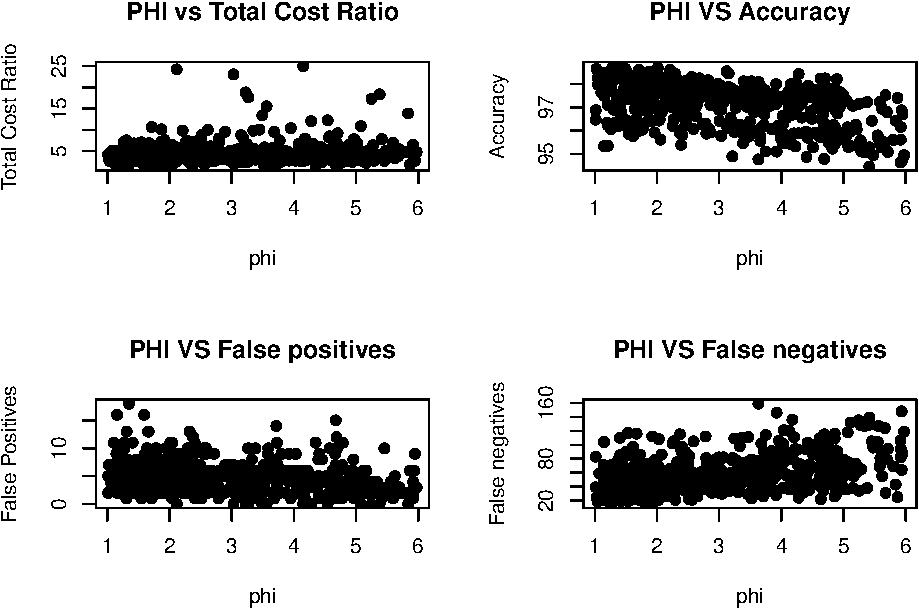
\includegraphics{spamizer_files/figure-latex/phi dispersion diagram-1.pdf}

\begin{Shaded}
\begin{Highlighting}[]
\KeywordTok{par}\NormalTok{(}\DataTypeTok{mfrow=}\KeywordTok{c}\NormalTok{(}\DecValTok{1}\NormalTok{,}\DecValTok{1}\NormalTok{))}
\end{Highlighting}
\end{Shaded}

En l'anterior grid podem veure diferents comparacions del comportament
de la variable phi sobre una mostra de 500 elements dins del conjunt
total de les execucions. Dels gràfics anteriors podem extreure certes
conclusions a vista tenint en compte que durant les execucions no s'ha
fixat en cap moment ni un ordre de lectura de correus, ni un valor per k
ni un valor per phi i els correus per validar eren seleccionats
aleatòriament. De totes maneres disposem d'un número molt elevat i amb
molta varietat de resultats.

\begin{itemize}
\tightlist
\item
  Es pot veure que la mitjana del tcr queda entre 1 i 6.
\item
  Es pot veure com a més valor de phi, més disminueix el nombre de fp
  (lentament).
\item
  Es pot veure com a més valor de phi més augmenta el nombre de fn (més
  pronunciat).
\item
  Es pot veure com l'accuracy es entre el 97 i 99 peró que si el valor
  de phi augmenta llavors l'accuracy baixa 4 punts.
\end{itemize}

\hypertarget{k}{%
\subsubsection{K}\label{k}}

Quan apliquem el suavitzat hem de tenir en compte què passa si donats el
bag of words de ham i el de spam una paraula no existeix. En la nostre
fòrmul aquest valor ens podria proporcionar multiplicacions per 0 i farà
que si una paraula no existeix aquesta paraula ja ens determini si un
correu és ham o és spam.

Per tant la k estipula el valor que se li assigna a una paraula quan
aquesta no és present. Aquest valor no pot ser 0 peró pot ser proper a
zero. Si fos zero es provocaria el mateix cas que l'esmentat
anteriorment. Tanmateix no té sentit aplicar un valor molt gran a la k
ja que si ho fem aquest valor provocaria que les paraules que no
existeixen fossin puntuades molt altes i se li treuria valor de còmput a
les aparicions.

\begin{Shaded}
\begin{Highlighting}[]
\KeywordTok{par}\NormalTok{(}\DataTypeTok{mfrow=}\KeywordTok{c}\NormalTok{(}\DecValTok{2}\NormalTok{,}\DecValTok{2}\NormalTok{))}
\KeywordTok{plot}\NormalTok{(m}\OperatorTok{$}\NormalTok{k, m}\OperatorTok{$}\NormalTok{tcr, }\DataTypeTok{main=}\StringTok{"k vs Total Cost Ratio"}\NormalTok{, }
   \DataTypeTok{xlab=}\StringTok{"k"}\NormalTok{, }\DataTypeTok{ylab=}\StringTok{"Total Cost Ratio"}\NormalTok{, }\DataTypeTok{pch=}\DecValTok{19}\NormalTok{)}

\KeywordTok{plot}\NormalTok{(m}\OperatorTok{$}\NormalTok{k, m}\OperatorTok{$}\NormalTok{accuracy, }\DataTypeTok{main=}\StringTok{"k VS Accuracy"}\NormalTok{, }
   \DataTypeTok{xlab=}\StringTok{"k"}\NormalTok{, }\DataTypeTok{ylab=}\StringTok{"Accuracy"}\NormalTok{, }\DataTypeTok{pch=}\DecValTok{19}\NormalTok{)}

\KeywordTok{plot}\NormalTok{(m}\OperatorTok{$}\NormalTok{k, m}\OperatorTok{$}\NormalTok{fp, }\DataTypeTok{main=}\StringTok{"k VS False positives"}\NormalTok{, }
   \DataTypeTok{xlab=}\StringTok{"k"}\NormalTok{, }\DataTypeTok{ylab=}\StringTok{"False Positives"}\NormalTok{, }\DataTypeTok{pch=}\DecValTok{19}\NormalTok{)}

\KeywordTok{plot}\NormalTok{(m}\OperatorTok{$}\NormalTok{k, m}\OperatorTok{$}\NormalTok{fn, }\DataTypeTok{main=}\StringTok{"k VS False negatives"}\NormalTok{, }
   \DataTypeTok{xlab=}\StringTok{"k"}\NormalTok{, }\DataTypeTok{ylab=}\StringTok{"False negatives"}\NormalTok{, }\DataTypeTok{pch=}\DecValTok{19}\NormalTok{)}
\end{Highlighting}
\end{Shaded}

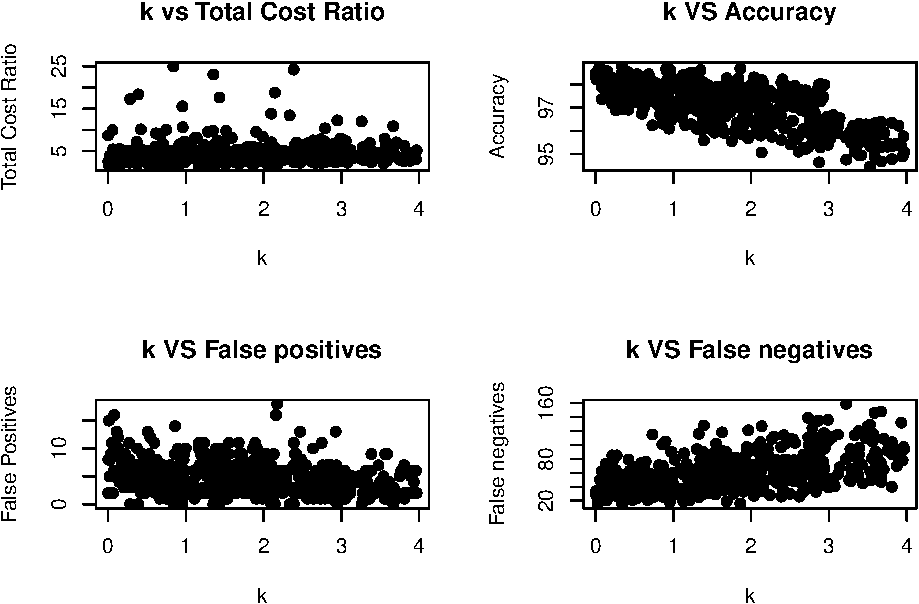
\includegraphics{spamizer_files/figure-latex/K dispersion diagram-1.pdf}

\begin{Shaded}
\begin{Highlighting}[]
\KeywordTok{par}\NormalTok{(}\DataTypeTok{mfrow=}\KeywordTok{c}\NormalTok{(}\DecValTok{1}\NormalTok{,}\DecValTok{1}\NormalTok{))}
\end{Highlighting}
\end{Shaded}

Utiitzant el mateix supòsit que en la variable phi observem doncs :

\begin{itemize}
\tightlist
\item
  Amb els valors de k per el tcr passa quelcom molt similar als valors
  de phi.
\item
  Amb els valors de k més petits l'accuracy ha augmenta, a mesura que es
  fa crèixer el valor de k més disminueix l'accuracy.
\item
  Veiem que no impacte molt aquest valor en el dels falços positius.
\item
  Per altra banda veiem que té una relació directe amb el comportament
  dels falços negatius. Limitarem els valors de k en un rang de (0 -
  1{]}.
\end{itemize}

\hypertarget{conlusions-conjuntes-entre-phi-i-k}{%
\subsubsection{Conlusions conjuntes entre phi i
k}\label{conlusions-conjuntes-entre-phi-i-k}}

No té sentit mirar les formes dels valors de phi i k de manera
independent per què son valors generats aleatòriament. El que sí que té
sentit és observar si les variables es poden descriure conjuntament amb
el nombre de FP o FN i finalment si es poden comprovar mitjançant el
total cost ratio. La variable phi està directament lligada amb els
valors FP i FN per definició.

Si fem gràfics en 3D dels valors de k i phi en funció del tcr
directament sobre la població d'execucions que tenim podem veure coses
interessants.

\begin{Shaded}
\begin{Highlighting}[]
\KeywordTok{par}\NormalTok{(}\DataTypeTok{mfrow=}\KeywordTok{c}\NormalTok{(}\DecValTok{1}\NormalTok{,}\DecValTok{2}\NormalTok{))}
\KeywordTok{scatter3D}\NormalTok{(v}\OperatorTok{$}\NormalTok{phi, v}\OperatorTok{$}\NormalTok{k, v}\OperatorTok{$}\NormalTok{tcr, }\DataTypeTok{phi =} \DecValTok{0}\NormalTok{, }\DataTypeTok{theta=}\DecValTok{0}\NormalTok{, }\DataTypeTok{bty =} \StringTok{"g"}\NormalTok{,  }\DataTypeTok{type =} \StringTok{"h"}\NormalTok{, }\DataTypeTok{ticktype =} \StringTok{"detailed"}\NormalTok{, }\DataTypeTok{pch =} \DecValTok{19}\NormalTok{, }\DataTypeTok{cex =} \FloatTok{0.5}\NormalTok{, }\DataTypeTok{xlab=}\StringTok{"PHI"}\NormalTok{, }\DataTypeTok{ylab=}\StringTok{"K"}\NormalTok{, }\DataTypeTok{zlab=}\StringTok{"TCR"}\NormalTok{)}
\KeywordTok{scatter3D}\NormalTok{(v}\OperatorTok{$}\NormalTok{phi, v}\OperatorTok{$}\NormalTok{k, v}\OperatorTok{$}\NormalTok{tcr, }\DataTypeTok{phi =} \DecValTok{0}\NormalTok{, }\DataTypeTok{theta=}\DecValTok{90}\NormalTok{, }\DataTypeTok{bty =} \StringTok{"g"}\NormalTok{,  }\DataTypeTok{type =} \StringTok{"h"}\NormalTok{, }\DataTypeTok{ticktype =} \StringTok{"detailed"}\NormalTok{, }\DataTypeTok{pch =} \DecValTok{19}\NormalTok{, }\DataTypeTok{cex =} \FloatTok{0.5}\NormalTok{, }\DataTypeTok{xlab=}\StringTok{"PHI"}\NormalTok{, }\DataTypeTok{ylab=}\StringTok{"K"}\NormalTok{, }\DataTypeTok{zlab=}\StringTok{"TCR"}\NormalTok{)}
\end{Highlighting}
\end{Shaded}

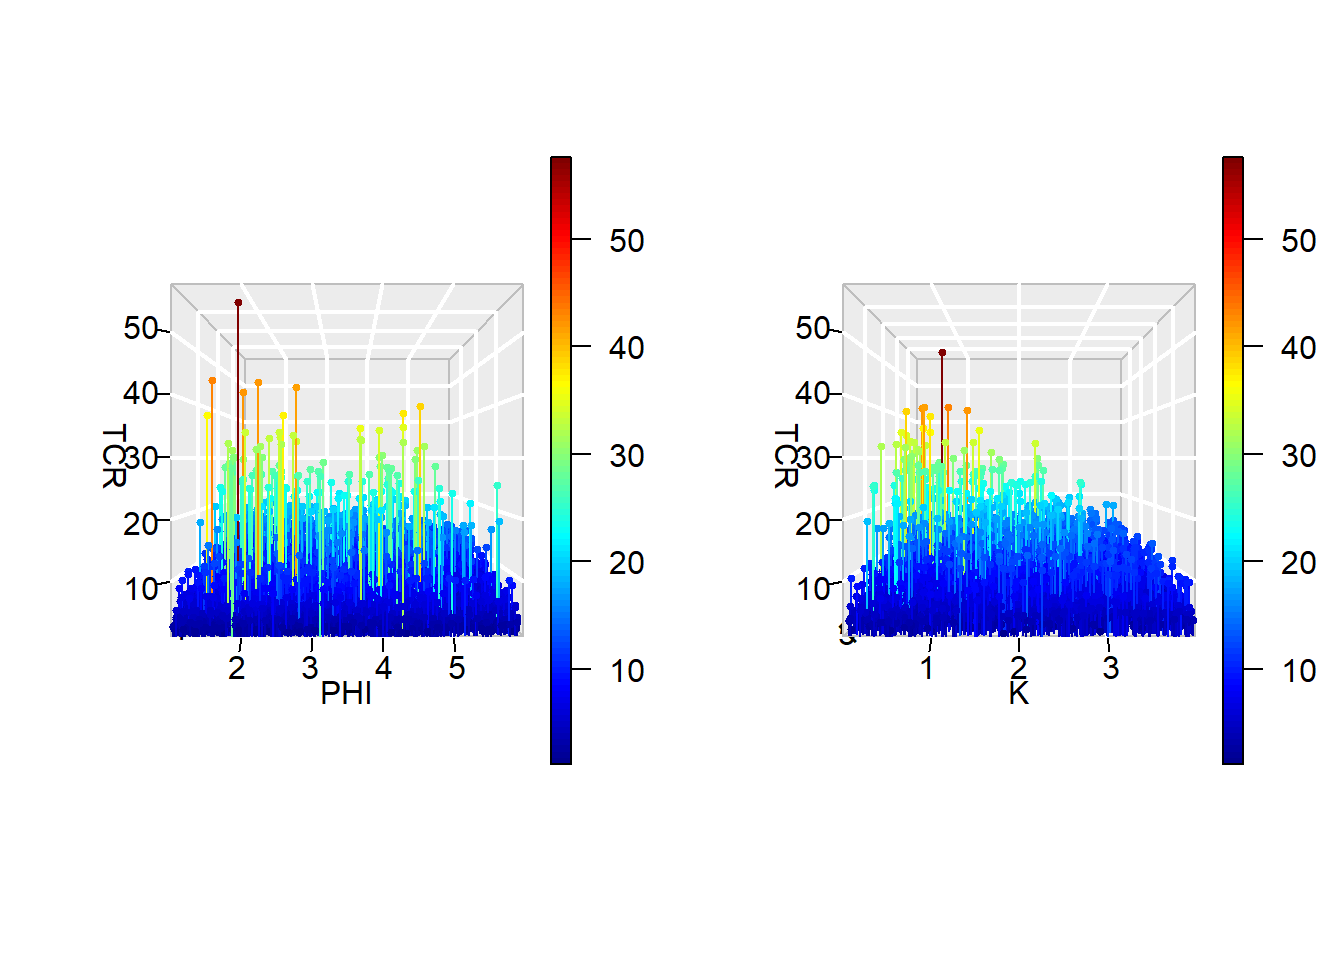
\includegraphics{spamizer_files/figure-latex/scatter-1.pdf}

\begin{Shaded}
\begin{Highlighting}[]
\KeywordTok{par}\NormalTok{(}\DataTypeTok{mfrow=}\KeywordTok{c}\NormalTok{(}\DecValTok{1}\NormalTok{,}\DecValTok{2}\NormalTok{))}
\KeywordTok{scatter3D}\NormalTok{(v}\OperatorTok{$}\NormalTok{phi, v}\OperatorTok{$}\NormalTok{k, v}\OperatorTok{$}\NormalTok{tcr, }\DataTypeTok{phi =} \DecValTok{0}\NormalTok{, }\DataTypeTok{bty =} \StringTok{"g"}\NormalTok{,  }\DataTypeTok{type =} \StringTok{"h"}\NormalTok{, }\DataTypeTok{ticktype =} \StringTok{"detailed"}\NormalTok{, }\DataTypeTok{pch =} \DecValTok{19}\NormalTok{, }\DataTypeTok{cex =} \FloatTok{0.5}\NormalTok{)}
\KeywordTok{scatter3D}\NormalTok{(v}\OperatorTok{$}\NormalTok{phi, v}\OperatorTok{$}\NormalTok{k, v}\OperatorTok{$}\NormalTok{tcr, }\DataTypeTok{phi =} \DecValTok{90}\NormalTok{, }\DataTypeTok{theta =} \FloatTok{0.5}\NormalTok{, }\DataTypeTok{bty =} \StringTok{"g"}\NormalTok{,  }\DataTypeTok{type =} \StringTok{"h"}\NormalTok{, }\DataTypeTok{ticktype =} \StringTok{"detailed"}\NormalTok{, }\DataTypeTok{pch =} \DecValTok{19}\NormalTok{, }\DataTypeTok{cex =} \FloatTok{0.5}\NormalTok{)}
\end{Highlighting}
\end{Shaded}

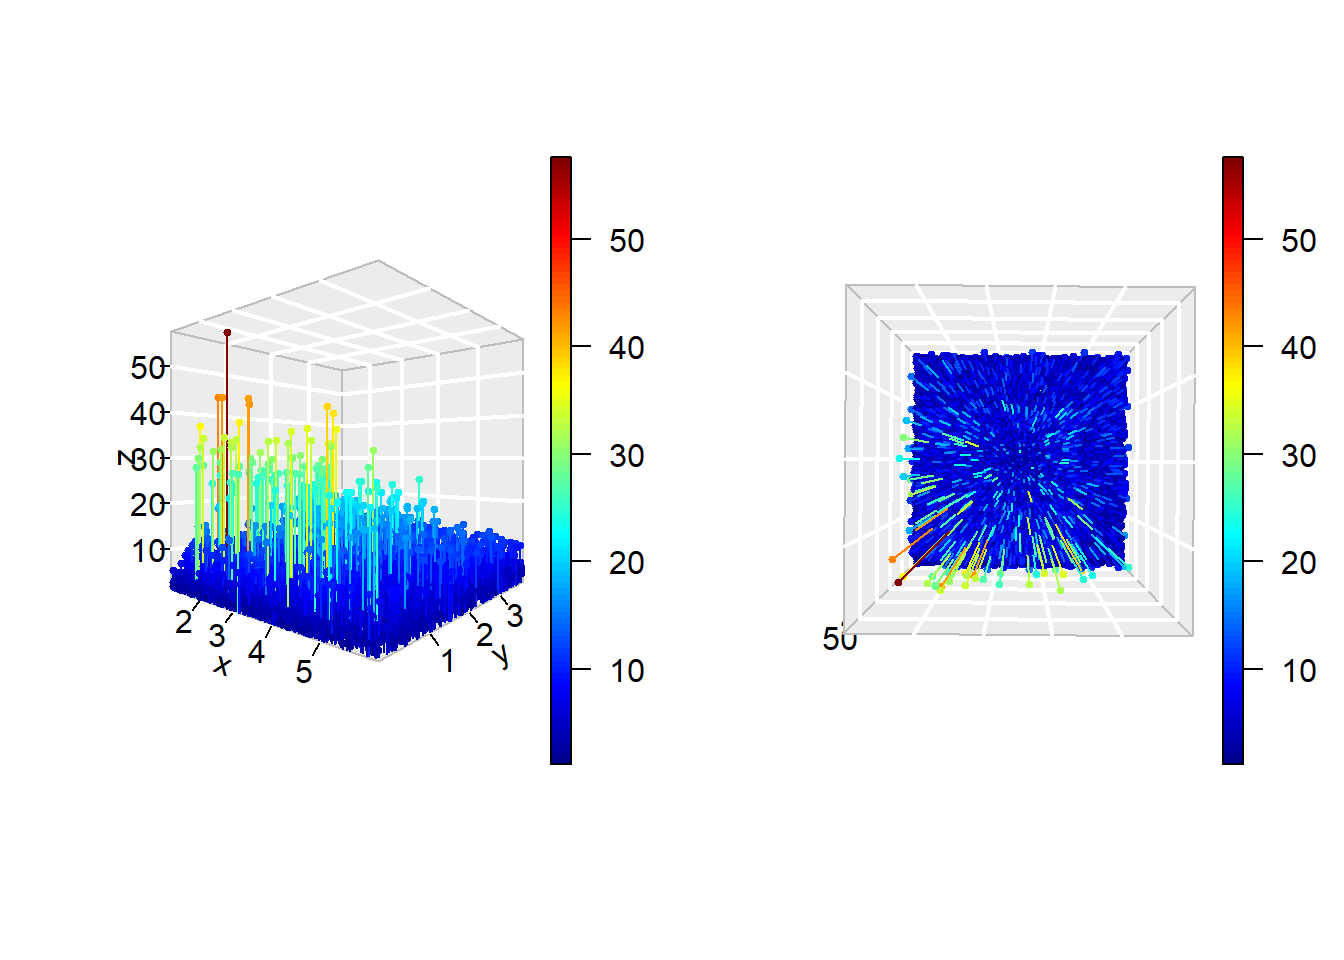
\includegraphics{spamizer_files/figure-latex/scatter-2.pdf}

En els anteriors gràfics es pot distingir perfectament el rang
d'actuació dels valors més alts per tcr. De la mateixa manera que s'ha
extret les conclusions sobre una mostra pensant que la mostra seria prou
representativa si observem sobre el total veiem que es confirmen les
conclusions que hem anat exposant.

Donat el valor de k entre 0 i 1 i els valors de phi també entre 0.5 i
2.5 és per on es mou el tant buscat màxim global de la funció conjunta.
Evidentment no hem formulat una hipòtesi concreta i no l'hem pogut
verificar ja que no hem ajustat el nostre model a cap mostra peró
utilitzant el coeficient de correlació de Pearson sobre els gràfics
mostrats per phi i per k en les seccions anteriors podem intuïr el
comportament de les variables.

No hem d'oblidar peró que el valor del tcr s'ha tret directament de
l'execució amb les variables phi i k i per tant ens serveix per veure si
hi ha algun patró pel que la funció k o la funció phi de manera
independent entre elles poden fer que creixi el valor del tcr, tanmatex
aixó no serà possible degut a que el valor del tcr s'extreu tant de la
variable phi tant com de la variable k i \textbf{S'hauria de fixar o bé
la phi o bé la k per poder extreure una conclusió sobre el tema}.

\hypertarget{referencies}{%
\subsection{Referències}\label{referencies}}

\begin{itemize}
\tightlist
\item
  \href{https://bl.ocks.org/patilv/raw/7360425/}{R graphics}
\end{itemize}


\end{document}
